\chapter{Diseño de la Solución}

% Contenidos basados en https://repositorio.uchile.cl/bitstream/handle/2250/191381/TablaConten.pdf?sequence=2&isAllowed=y
La aplicación creada, llamada IGACSE (Interactive Graph Algorithms for Computer Science Education) de ahora en adelante, es propuesta y diseñada en base a algunos requerimientos y necesidades de los estudiantes de computación que se nombrarán en las siguientes secciones.

\section{Referentes}

Los referentes más importantes son aquellos videojuegos que tienen un rol educativo relacionado a la programación, como CodeCombat \ref{CodeCombat} y 7 Billion Humans \ref{7BillionHumans}.

Se observa que estos juegos tienen una componente textual que destaca en la interfaz del juego principal, ocupando al menos el 20\% de la pantalla. Por otra parte, hay texto que avanza en una línea narrativa al inicio y final de cada nivel.

En ambos casos la interfaz de código se encuentra a la derecha. Además, estos juegos permiten mostrar al usuario cómo la ejecución de las instrucciones afecta al juego paso a paso.

De este análisis se desprende que el juego tiene por requisito mostrar la ejecución del código instrucción por instrucción.

\section{Objetivo del diseño deseado}

En este apartado se justifican las decisiones de diseño que llevaron a las mecánicas de juego, cuáles son los elementos interactivos y la ubicación y responsividad de estos. Según Rogers en su libro sobre diseño interactivo \cite{Rogers2002InteractionDesign}, es relevante entender primero cuál es el problema que busca resolverse, qué usuarios se ven afectados por esto, qué características poseen y cómo podría solucionarse en base a prototipos.

Se parte del supuesto de que, en muchas ocasiones, los estudiantes creen entender cómo funciona cierto código o algoritmo, pero no lo aplican paso a paso con papel y lápiz o en su imaginación propia. Cuando se les asigna como ejercicio realizar el procedimiento siguiendo cada instrucción rigurosamente, los estudiantes no lo llevan a cabo o lo hacen de forma incorrecta sin darse cuenta. Por ejemplo, en \cite{IdentifyingStudentDifficultiesDataStructures}, se menciona que los estudiantes a menudo creen entender los contenidos, pero tienen conceptos erróneos sin percatarse.

En el trabajo de Zingaro et al. \cite{IdentifyingStudentDifficultiesDataStructures}, se mencionan algunos ejemplos de malentendidos por parte de los estudiantes, como errores al comprender los heaps y las formas en que pueden representarse o construirse. Estos malentendidos pasan desapercibidos y no son detectables por los mismos estudiantes.

Adicionalmente a la revisión de textos, se revisaron canales de YouTube educativos como 3Blue1Brown \cite{3Blue1BrownYT}, donde el propietario del canal, Grant Sanderson, habla repetidamente sobre cómo las visualizaciones ayudan a comprender la abstracción matemática subyacente.

Un requisito esencial es que el videojuego logrado debe evitar la mecanización por parte del estudiante, obligándolo a revisar exhaustivamente cada paso relacionado con el algoritmo, evitando dar por sentado que se entiende el código y saltar a la siguiente actividad.

Por otra parte, para enseñar conceptos relacionados con programación, lo ideal es buscar usuarios que entiendan cómo funciona, pero que no tengan mucha experiencia y que no visualicen un código al nivel de entender cómo funciona instrucción por instrucción. Por lo mismo, se propone basarse en un modelo similar a los debuggers, donde se puede ver el estado de las variables en cada paso, así como la instrucción por ejecutarse y el resultado que conlleva.

\section{Descripción de la aplicación al momento de la realización de los experimentos}

El videojuego se separa en distintos niveles. Consta de un menú principal, tutoriales y niveles jugables. En el menú principal se puede seleccionar el nivel a jugar o un modo historia. En el modo historia, se juegan todos los niveles en orden, y se desbloquean a medida que se avanza.

En los tutoriales se abordan los conceptos básicos de grafos sin indicar explícitamente al usuario qué es un grafo. Además, se enseñan conceptos de jugabilidad, como explorar o seleccionar un nodo, navegar en el código ejecutando instrucciones y responder preguntas del tipo Sí/No cuando el código incluye una instrucción con un if.

Finalmente, se presentan los niveles jugables, correspondientes a los algoritmos que se buscan enseñar: BFS (Breadth First Search) y DFS (Depth First Search). En estos niveles, no se presenta una historia y hay menos ayuda para el usuario. Una vez completados los niveles jugables, se mostrarán los créditos del juego.

El juego se centra en explorar planetas a través de rutas, utilizando una metáfora de grafos, donde los planetas representan nodos y los caminos entre ellos son aristas. El objetivo es rescatar pandas rojos dispersos en los planetas. Para lograrlo, es necesario explorar todos los nodos en una galaxia, correspondiente a un nivel. En cada nivel, se enseña un algoritmo distinto.

El juego guía al usuario mediante instrucciones que aparecen en el lado derecho de la pantalla. El jugador pasa a la siguiente instrucción presionando la tecla de espacio. Cada vez que avanza a la siguiente instrucción, se desencadenan efectos y animaciones que muestran qué está sucediendo en el código. Estas animaciones se reflejan en el viewport del juego, donde se destaca un planeta, un camino o una nave que se desplaza hacia otro planeta.

En los tutoriales se enseñan los conceptos básicos de grafos, pero sin indicarle al usuario explícitamente qué es un grafo. Además, se enseñan conceptos de jugabilidad, cómo explorar o seleccionar un nodo, cómo navegar en el código ejecutando instrucciones, y cómo contestar preguntas del tipo Sí/No cuando el código tiene una instrucción que incluya un if.

Al seguir las instrucciones en su totalidad, el jugador repite el algoritmo paso a paso, lo que le permite entender cómo funciona y cuál es su finalidad.

Las acciones del jugador pueden ir acompañadas de un sonido recompensante, permitiéndole avanzar a la siguiente instrucción. En caso de cometer un error, se indicará al jugador mediante una animación visual y un sonido. Si el jugador no sabe qué hacer, en ciertos casos se mostrará un hint visual indicándole que debe presionar alguna tecla específica o hacer clic en algún planeta.


\subsection{Diagrama de flujo de juego}

El juego inicia mostrando el menú principal, donde se puede seleccionar el modo historia o los niveles jugables. Si se elige el modo historia, se mostrarán los tutoriales. Una vez terminados los tutoriales, se mostrará el primer nivel jugable, que es DFS. Si se eligen los niveles jugables, se mostrarán los niveles jugables, donde se puede seleccionar el nivel a jugar, BFS o DFS.
Terminados los niveles BFS y DFS, se mostrarán los créditos.

\begin{figure}[h]
	\centering
	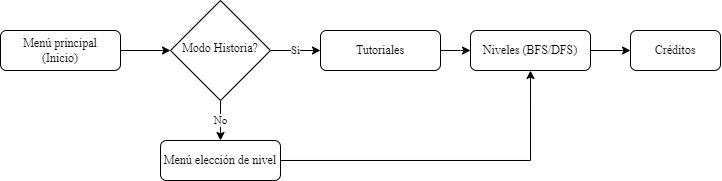
\includegraphics[scale=.5]{imagenes/FlujoDeJuego.png}
	\caption{ Flujo de juego de IGACSE}
	\label{FlujoDeJuego}
\end{figure}


\subsection{Narrativa}

La narrativa se desarrolla en el espacio exterior, donde una nave inicia un diálogo con una estación llamada DCC. La misión de la nave es rescatar pandas rojos dispersos en los planetas de la galaxia. En un inicio, el piloto señala que los niveles de combustible son bajos, y la estación sugiere continuar con las siguientes galaxias, evitando el uso del piloto automático debido al alto costo y consumo de combustible de las redes neuronales. Para optimizar recursos, la nave deberá seguir instrucciones manuales para completar la misión.

Con cada galaxia visitada, el piloto rescata y encuentra otros pandas rojos. Se premia al jugador para que siga con los siguientes niveles y que termine el juego. Los pandas rojos son la mascota del Centro de Alumnos del Departamento de Ciencias  de la Computación (CADCC).  Durante las actividades de bienvenida a los nuevos estudiantes, se muestran afiches con esta mascota \cite{CADCCPage}, por lo que se busca que el jugador se sienta identificado con el juego. Además, la estación se llama DCC para aumentar el sentido de identificación con el jugador, pues DCC son las siglas del Departamento de Ciencias de la Computación \cite{DCCPage}.


\subsection{Menú principal}

En el menú principal, se puede seleccionar el idioma presionando el botón en la esquina superior izquierda de la figura \ref{MenuPrincipal}. Los idiomas disponibles son inglés y español. Además, ofrece las opciones para jugar en el modo historia o los niveles jugables.

\begin{figure}[h]
	\centering
	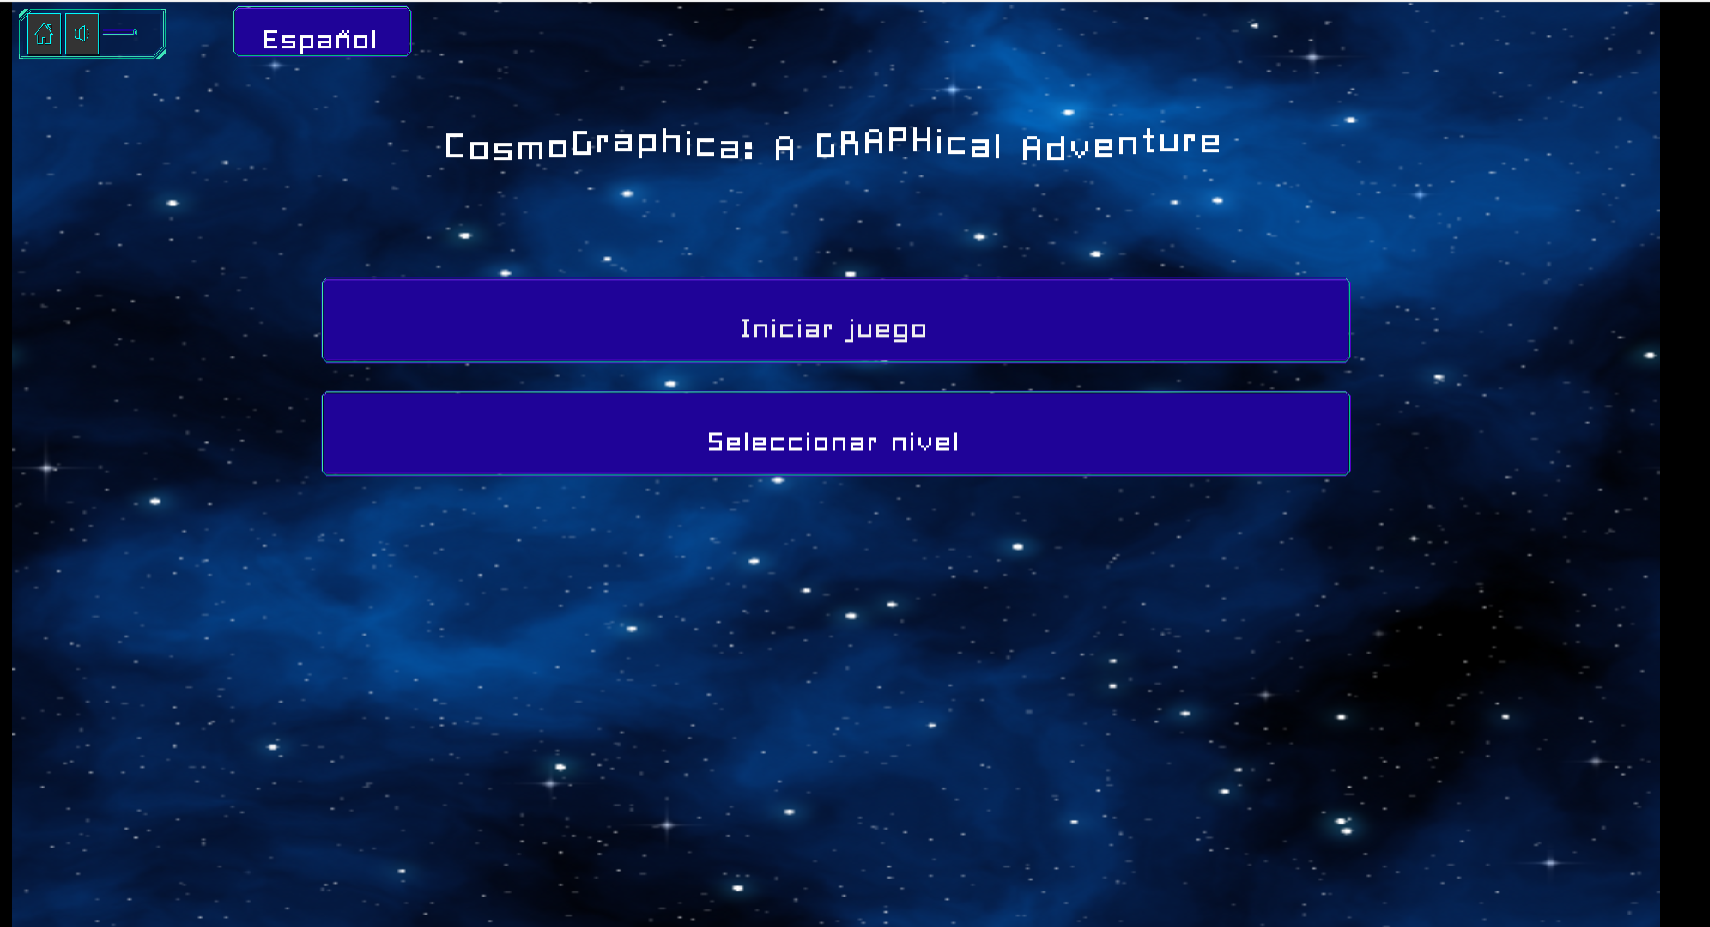
\includegraphics[scale=0.3]{imagenes/MainMenu.png}
	\caption{Menú principal de IGACSE, que se muestra al iniciar el juego.}
	\label{MenuPrincipal}
\end{figure}


\subsection{Tutoriales}

Los tutoriales tienen como objetivo familiarizar al jugador con las mecánicas básicas que se utilizarán a lo largo del juego. Además, introducen al jugador en la historia, ambientada en una nave que rescata pandas rojos dispersos en los planetas de la galaxia. La trama busca ilustrar la aplicación de los grafos sin detallar explícitamente el contenido que se está enseñando. Las mecánicas se presentan mediante una combinación de elementos, como texto y pistas visuales, que pueden incluir un ratón realizando clic izquierdo o una tecla R siendo presionada sobre el planeta. Cada nivel y tutorial son repetibles, permitiendo al jugador revisarlos en caso de no comprender algún aspecto.

\subsubsection{Primer Tutorial}

En el primer tutorial, se pretende familiarizar al jugador con la pantalla, demostrando que los planetas son navegables y que existen caminos que los conectan, permitiendo hacer clic entre ellos. En esta etapa, también se proporciona información sobre el diálogo y se presentan pistas visuales.


\begin{figure}[h]
	\centering
	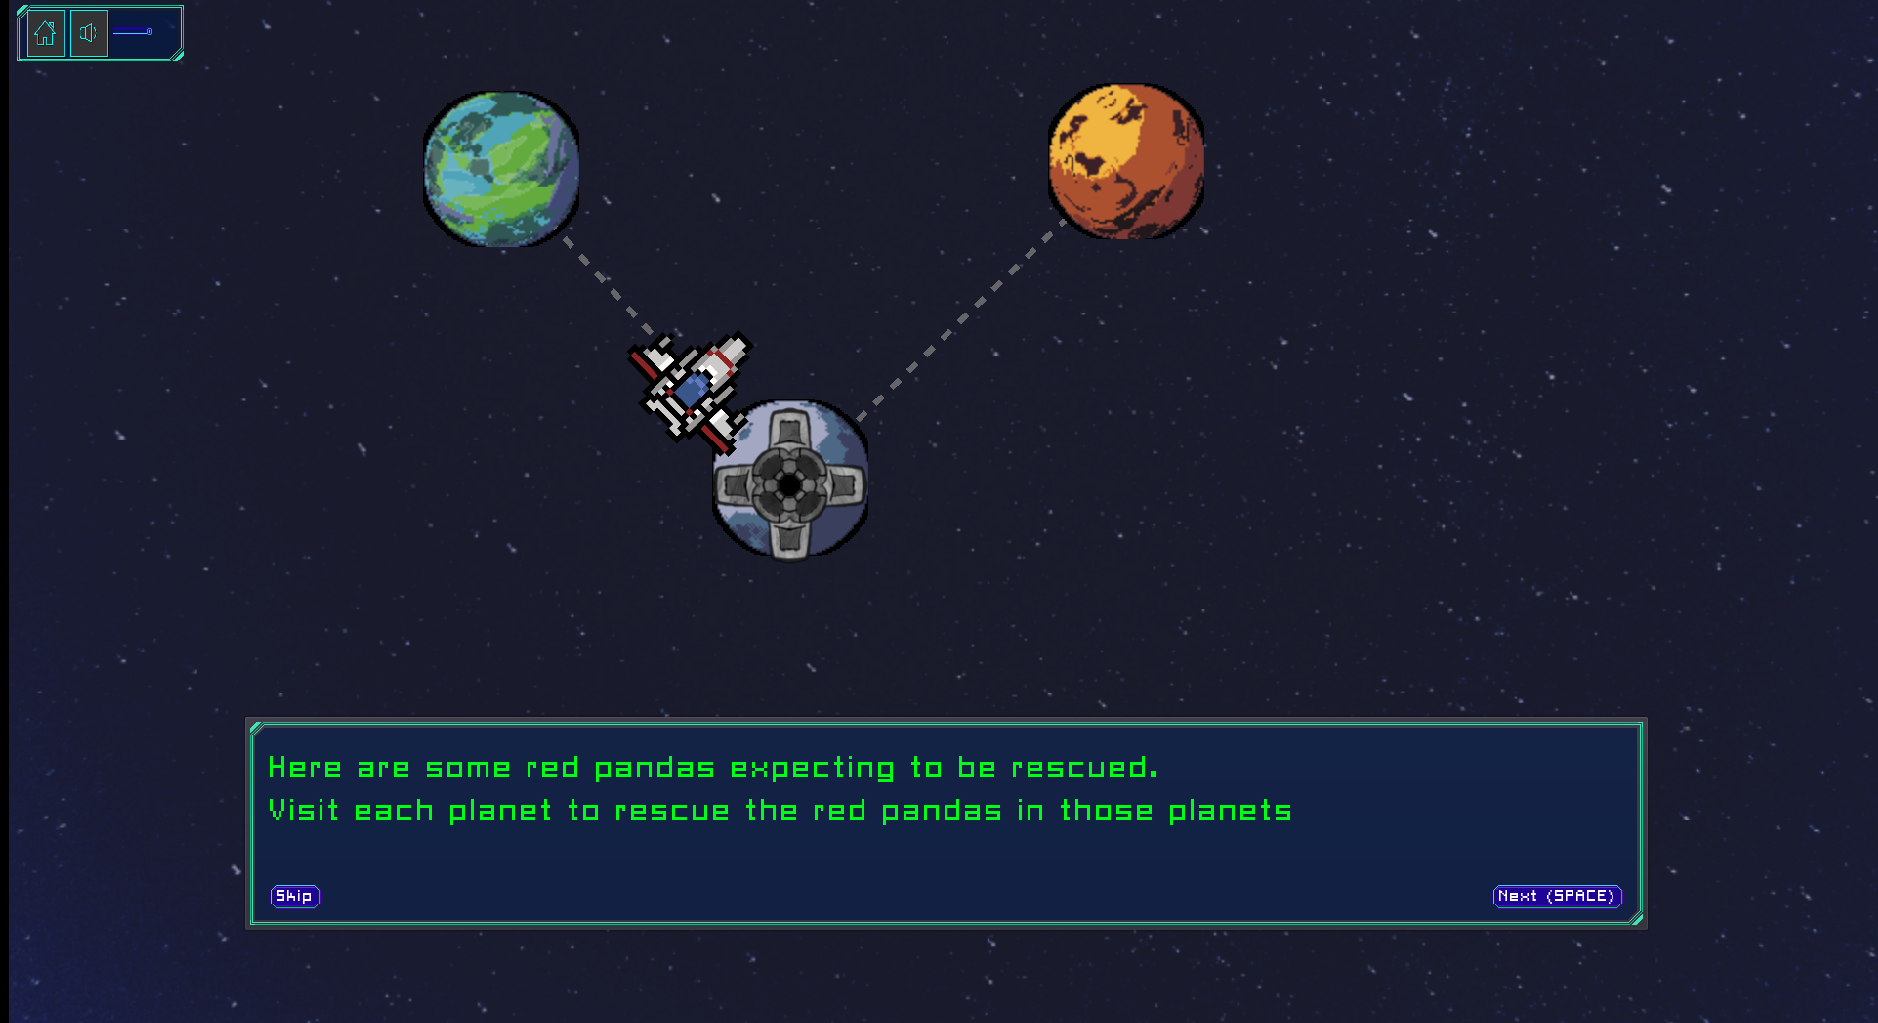
\includegraphics[scale=0.3]{imagenes/FirstTutorial.png}
	\caption{Primer tutorial. Se le indica al jugador a través de un diálogo que debe visitar cada planeta.}
	\label{FirstTutorial}
\end{figure}



\subsubsection{Segundo tutorial}

En el segundo tutorial, se presenta la mecánica de instrucciones e introduce el ciclo for y el if en las instrucciones, elementos que se utilizarán más adelante.

Al inicio del segundo tutorial, se le indica al jugador que debe seguir las instrucciones del algoritmo debido a que la exploración automatizada de los pandas rojos es costosa y el combustible se está agotando. Las primeras dos instrucciones solicitan al jugador que presione la tecla espacio para avanzar a la siguiente instrucción (ver figura \ref{SecondTutorial}).


\begin{figure}[h]
	\centering
	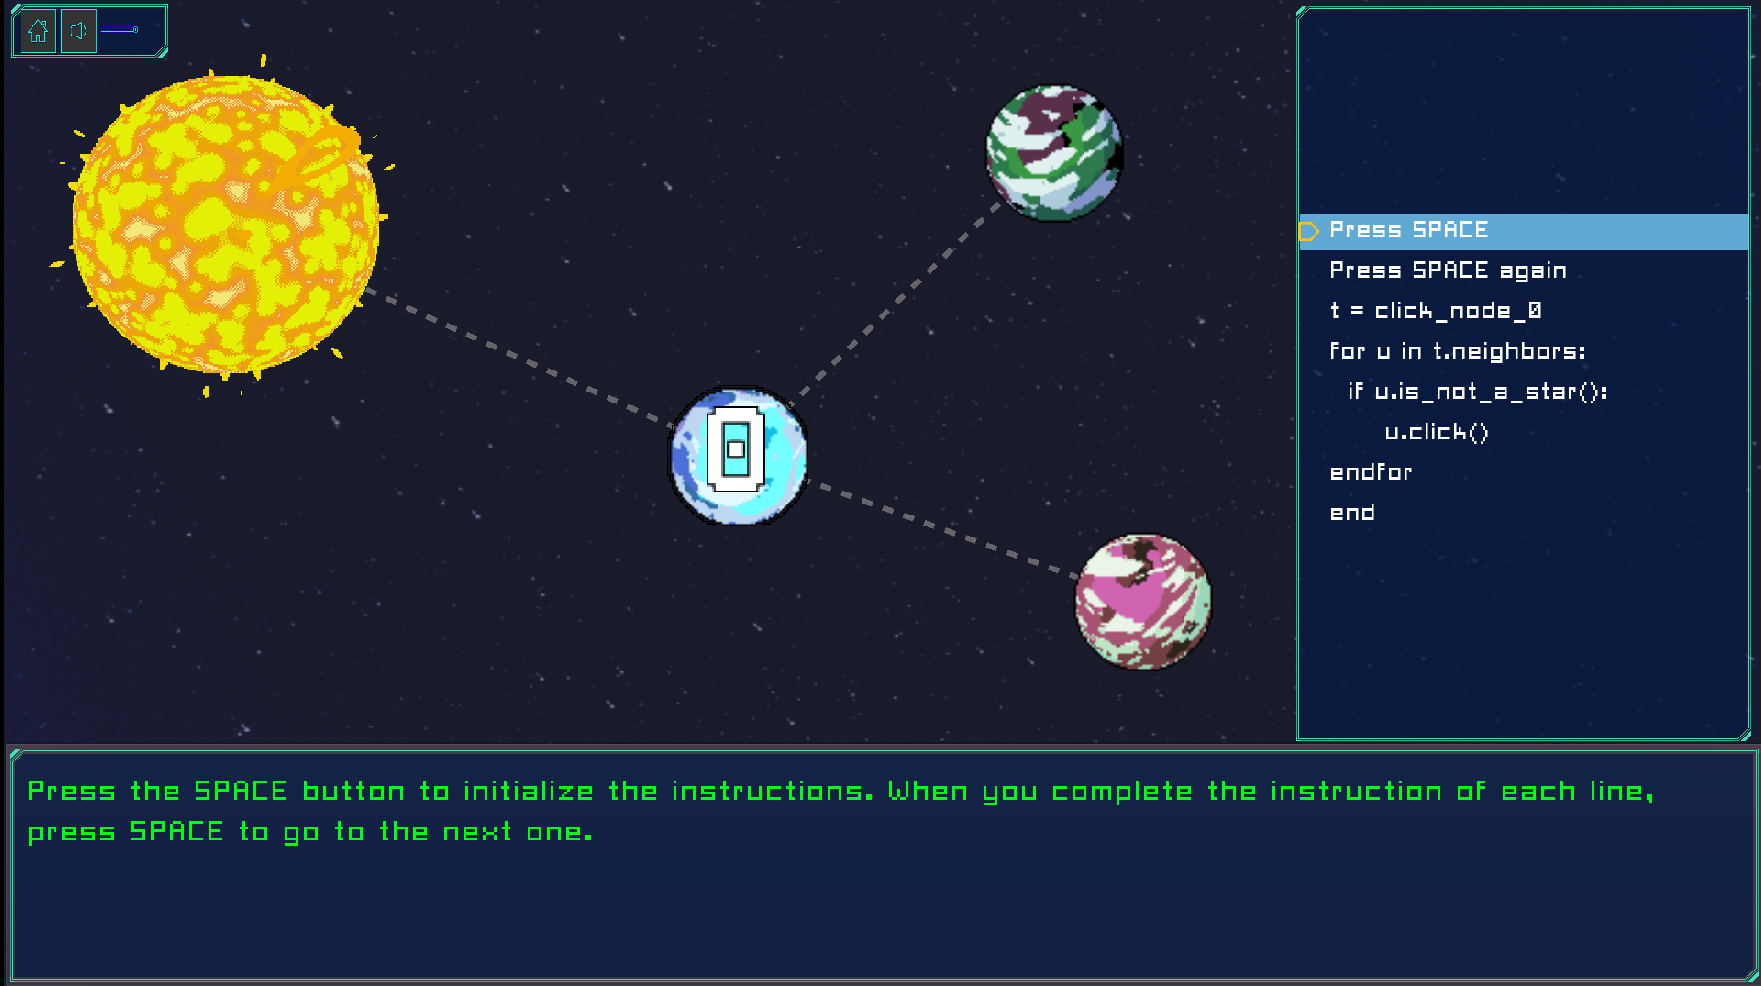
\includegraphics[scale=0.2]{imagenes/SecondTutorial.png}
	\caption{Segundo tutorial. Se le muestra un diálogo de entrada al jugador introduciéndole el nuevo concepto. Este es el primer momento en que se le muestran las instrucciones al jugador.}
	\label{SecondTutorial}
\end{figure}

Durante este segundo tutorial, se introduce la lógica de responder sí o no cuando aparece una instrucción con un if. El jugador debe dar la respuesta correcta para avanzar a la siguiente instrucción. Si responde incorrectamente, perderá y deberá reiniciar el nivel. En la figura \ref{SecondTutorialShowingIf}, se muestra la ventana que aparece al jugador al llegar a una instrucción con un if.

\begin{figure}[h]
	\centering
	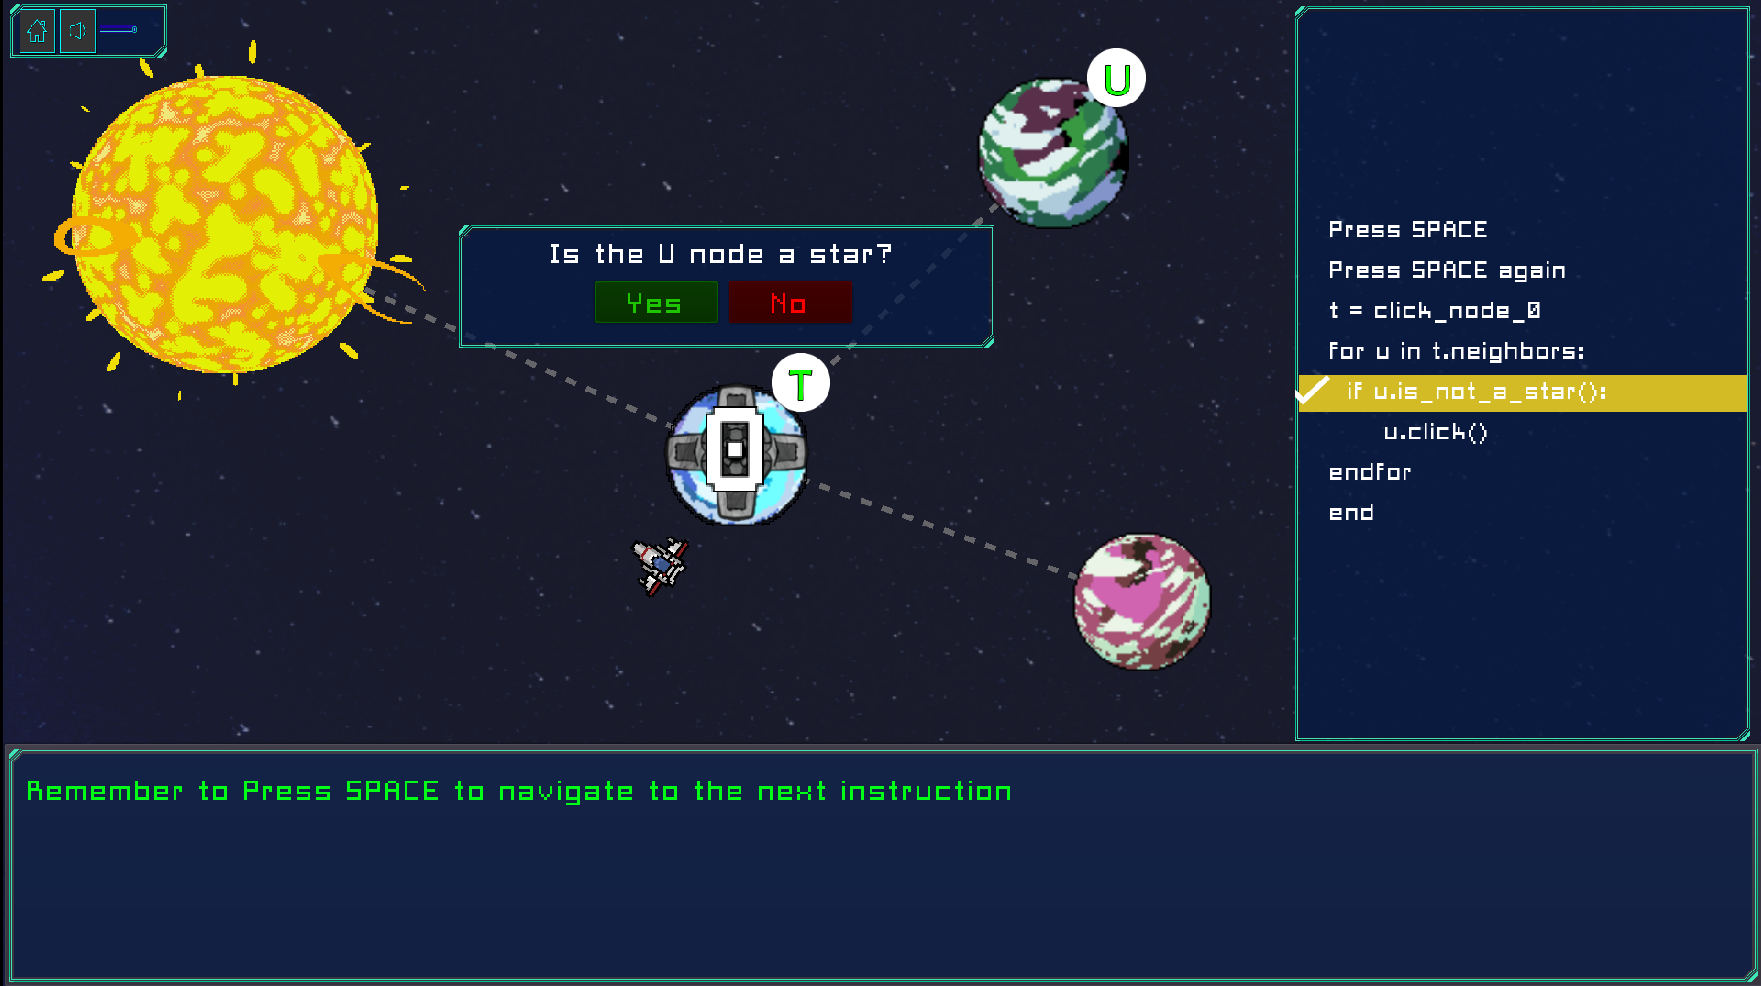
\includegraphics[scale=0.3]{imagenes/SecondTutorialShowingIf.png}
	\caption{Segundo tutorial. Ventana de if que le aparece al jugador al llegar a una instruccion con un if. El jugador debe responder sí o no correctamente para avanzar}
	\label{SecondTutorialShowingIf}
\end{figure}

\subsubsection{Tercer tutorial}

El tercer tutorial introduce al jugador el concepto de Pilas (Stacks) y Colas (Queues) como estructuras de datos para almacenar nodos y luego obtenerlos en órdenes distintos. Además, se le introduce al jugador sobre las variables creadas y la variable seleccionada, la cual se usa para señalar a qué objeto se le agregará el nodo que el usuario presione.

\begin{figure}[h]
	\centering
	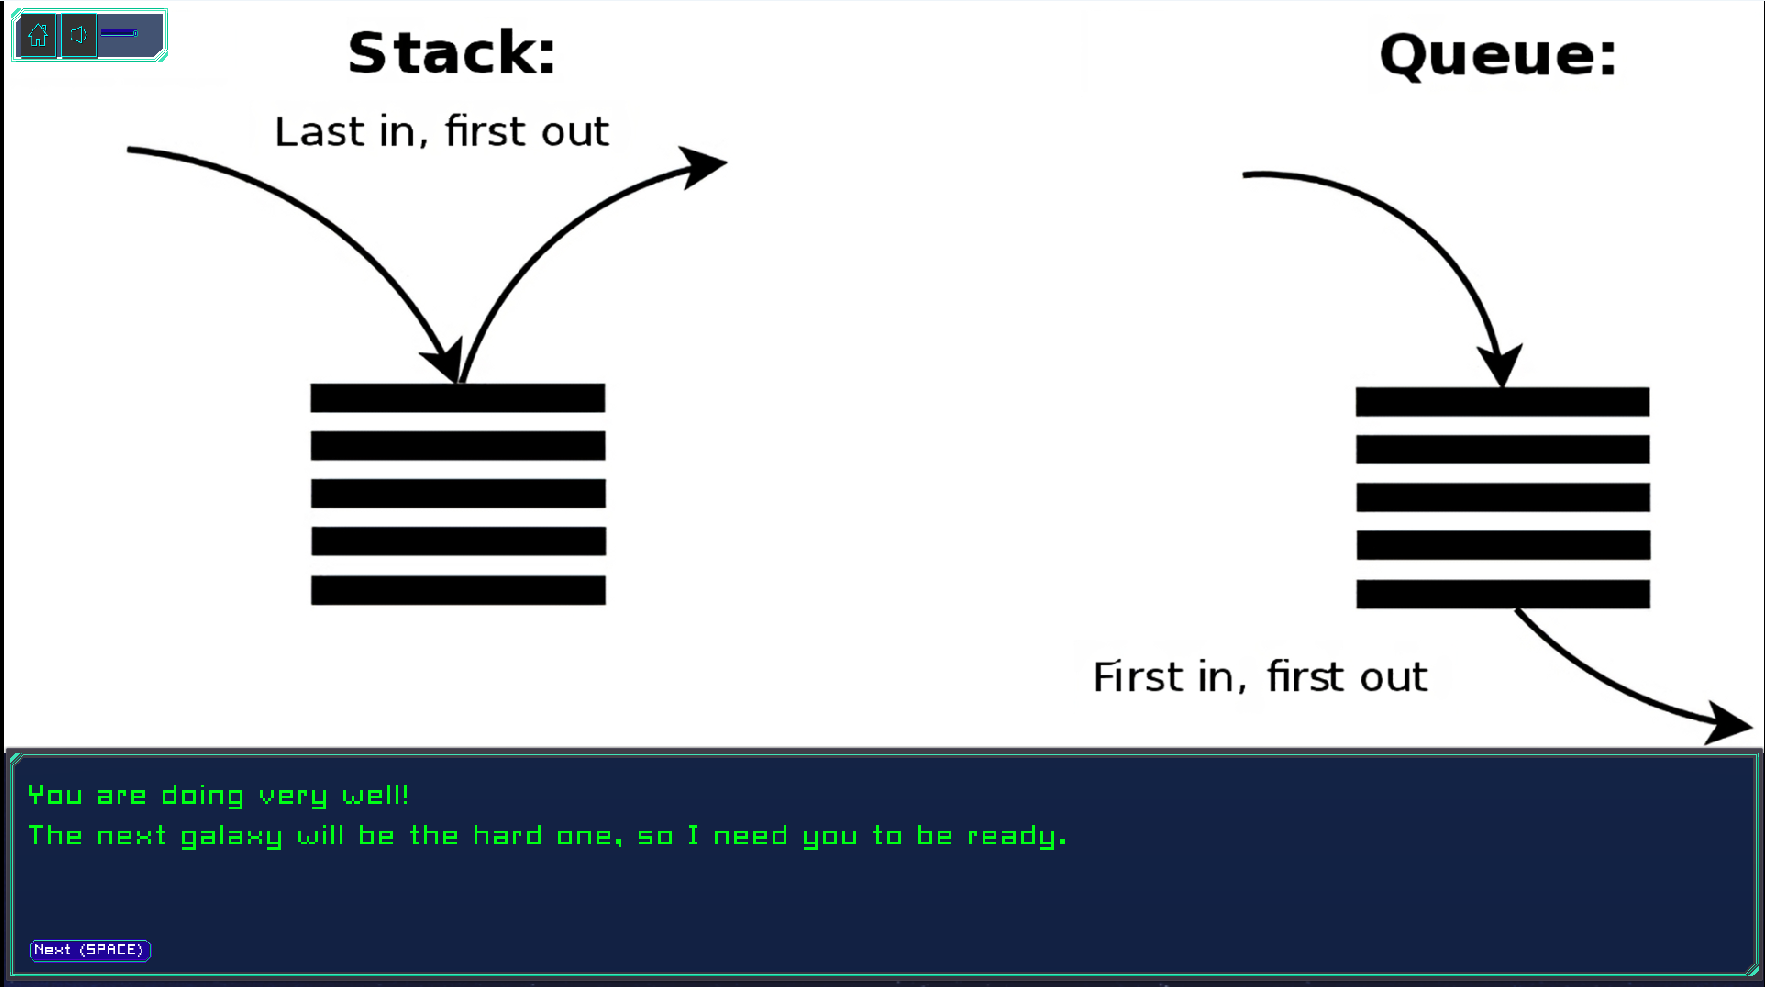
\includegraphics[scale=0.3]{imagenes/ThirdTutorialFirstDialogue.png}
	\caption{Tercer tutorial. Se le explica al usuario al inicio qué son las colas y stacks y cómo funcionan y en qué difieren.}
	\label{ThirdTutorialFirstDialogue}
\end{figure}


\begin{figure}[h]
	\centering
	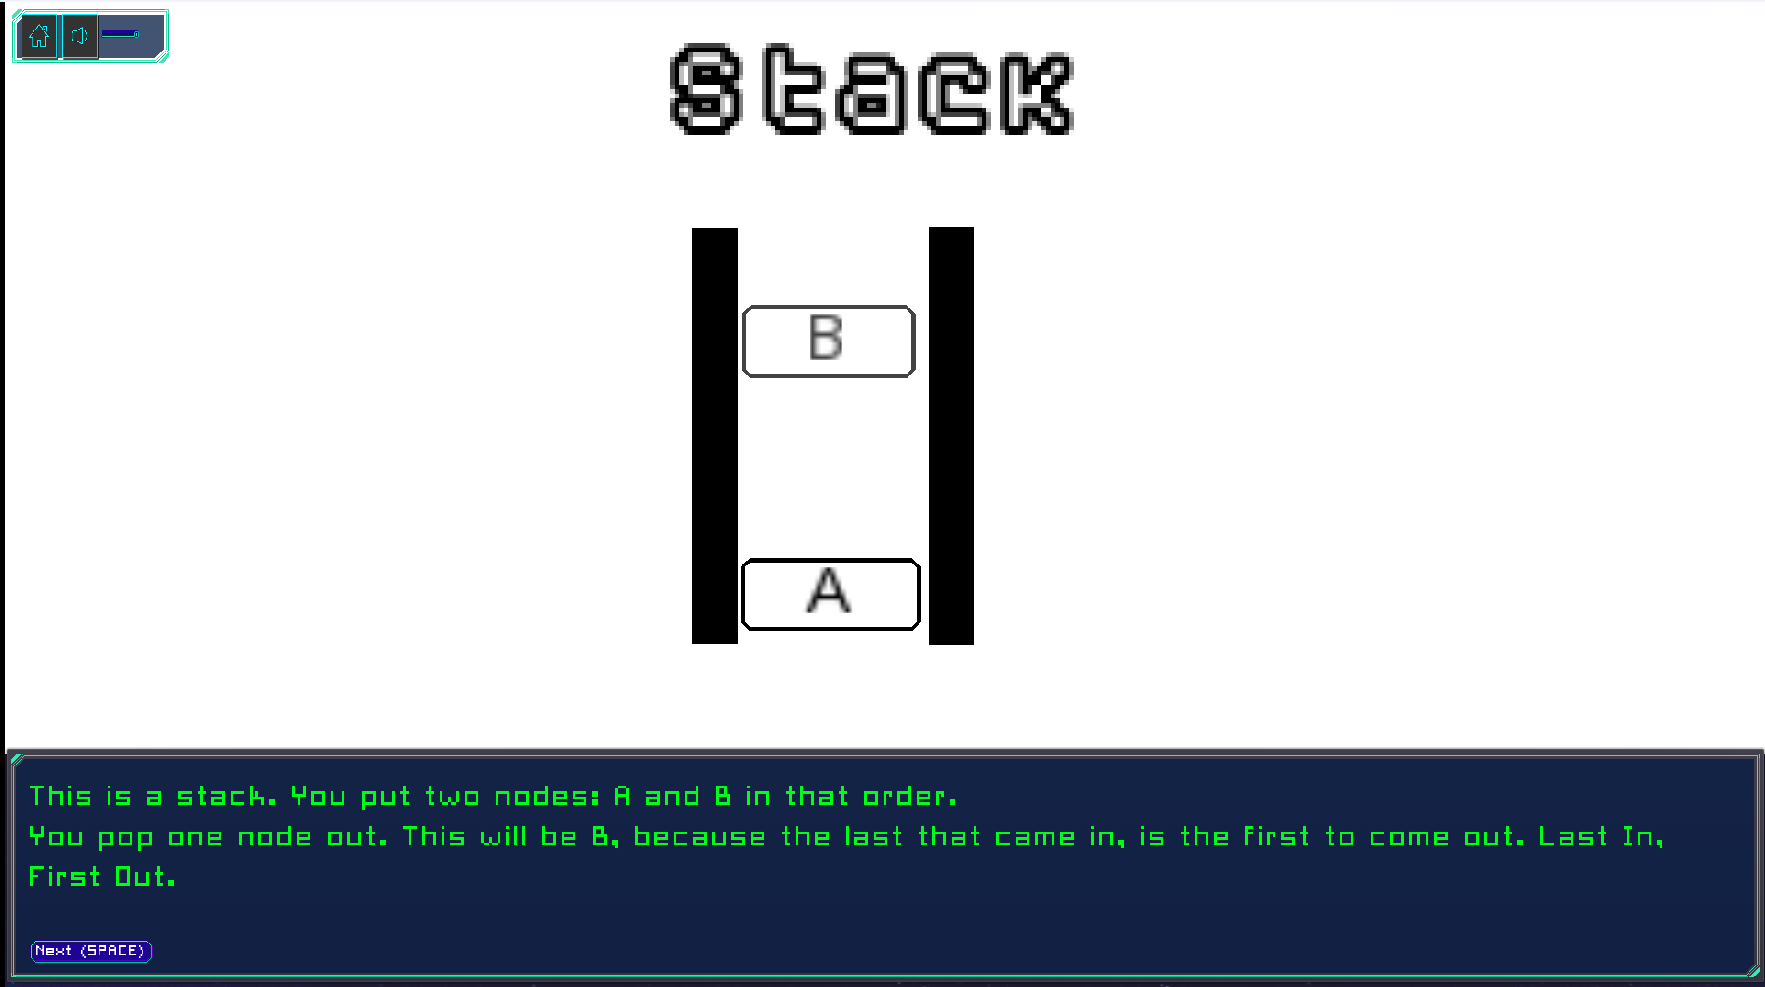
\includegraphics[scale=0.3]{imagenes/ThirdTutorialStackExplanation.png}
	\caption{Tercer tutorial. Mostrando al usuario cómo funciona un stack a través de animaciones.}
	\label{ThirdTutorialStackExplanation}
\end{figure}


El objetivo de las instrucciones en este tutorial es que el jugador aprenda la mecánica para agregar nodos a un stack o a una pila. Además, se refuerza la mecánica de las instrucciones y ejecutar cada acción paso por paso.


\begin{figure}[h]
	\centering
	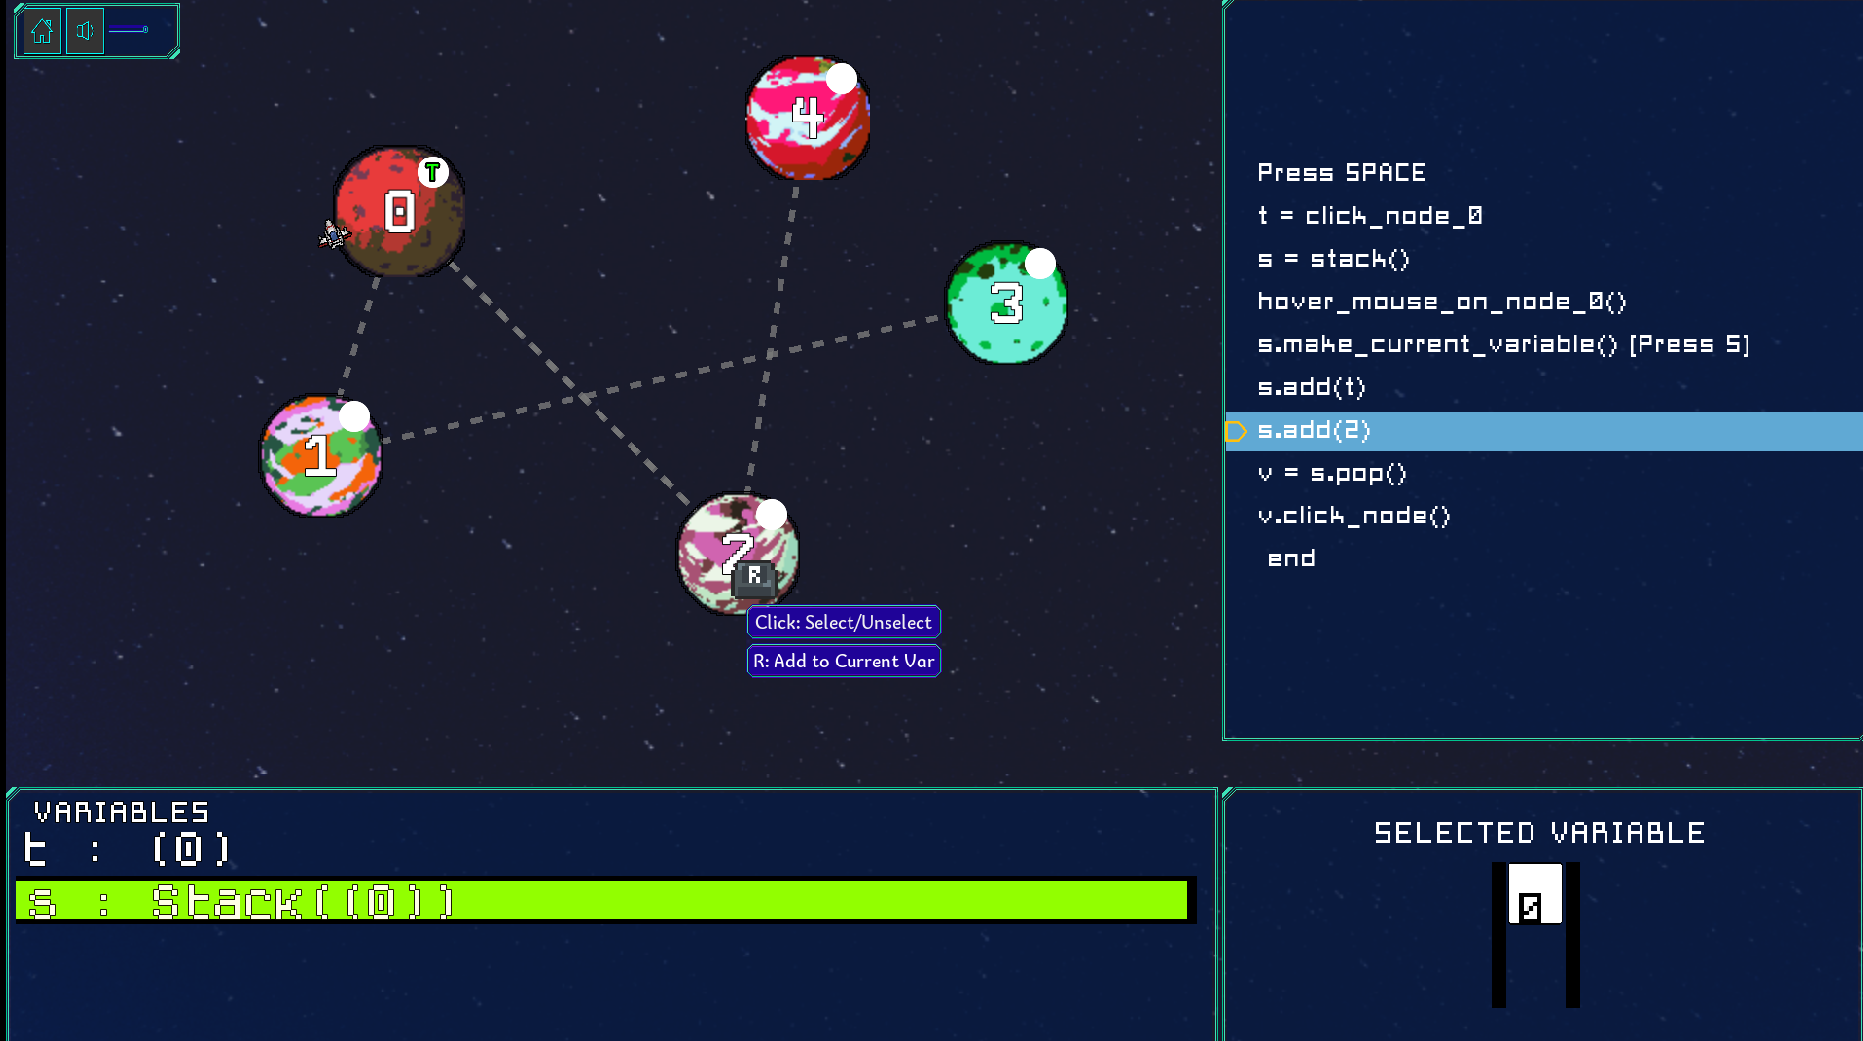
\includegraphics[scale=0.3]{imagenes/ThirdTutorialAddingNode.png}
	\caption{Tercer tutorial. El jugador debe presionar R sobre el planeta 2 para avanzar a la siguiente instrucción.}
	\label{ThirdTutorialAddingNodesToStacks}
\end{figure}


\subsection{Niveles jugables}

Los niveles jugables presentados son BFS y DFS, que enseñan esos algoritmos. Los planetas y sus conexiones son aleatorias, con la restricción de que el grafo formado es siempre conexo, es decir, todos sus nodos tienen al menos un camino hacia el resto de los otros nodos.

Se crearon 4 niveles para el juego, incluyendo los algoritmos de Kruskal y Prim. Sin embargo, estos últimos no fueron incluidos en la versión final del juego, pues el diseño y la experiencia de usuario eran distintos por requerir otro tipo de acciones, como ordenar arcos y operar con conjuntos, obteniendo uniones e intersecciones. Además, el tiempo de la prueba de usuario era aproximadamente de 45 minutos, por lo que se prefirió no incluirlo en la prueba dado que no se contaba con el tiempo suficiente para probarlos.


\section{Proceso de diseño}

Para diseñar el videojuego, primero se determinaron problemas que se querían solucionar. En particular, el autor hipotetiza que los estudiantes de computación tienen dificultades para comprender completamente los algoritmos que se enseñan en los cursos de programación, y que no siempre son conscientes de esta falta de comprensión. Por lo tanto, se busca que este videojuego sea una herramienta que permita a los estudiantes entender los algoritmos paso a paso, guiándolos sutilmente a lo largo del proceso de aprendizaje.

En la Universidad de Chile, históricamente y al momento de realizar este trabajo, para entrar a computación se requiere aprobar anteriormente dos años de cursos de plan común, donde existe una práctica conocida como ``pauteo'', la cual consiste en estudiar y revisar pautas de pruebas de semestres pasados para preparase para los exámenes. Con esta práctica, el alumnado revisa las ecuaciones o procedimientos para responder una pregunta sin haber realizado los ejercicios o repetido el procedimiento paso por paso. Muchas veces revisan un algoritmo superficialmente, o lo reproducen mentalmente sin hacerlo en papel. Por lo mismo, se busca que el videojuego sea una herramienta que permita a los estudiantes entender los algoritmos paso a paso y acompañarlo con una visualización.

La idea principal es forzar al usuario a reproducir el algoritmo paso a paso. Esto se puede observar al utilizar el debugger. El debugger permite ver el estado de las variables en cada paso, y permite avanzar paso a paso en el código. El videojuego busca ser una herramienta que permita al usuario reproducir el algoritmo paso a paso, pero de una manera más lúdica. Por esto, el debugger que se utiliza en Visual Studio Code se utilizó como modelo.

% Agregar imagen de debugger en VSCode con un código de Python.

Posteriormente, se realizaron distintos bocetos. Se le mostraron estos bocetos a un diseñador de videojuegos profesional con títulos ya liberados. Se eligió el que fue entendido a primera vista y que se veía más atractivo, además que se parecía más a Visual Studio Code. Se implementaron versiones del videojuego con Godot, que permitía agregar nuevas funcionalidades rápidamente, además de permitir cambiar el estilo. El autor del trabajo mostraba su trabajo de tesis semana a semana en un curso de 20 estudiantes, donde se recibían comentarios del resto de los alumnos.

Una vez definido cierto nivel de avance con todos los algoritmos definidos, se probó con 4 usuarios expertos que ya conocían el algoritmo. Sin embargo, no fueron capaces de seguirlo o comprenderlo a cabalidad, por lo que no se cumpliría el objetivo con personas neófitas en los grafos. Por esta razón, se decidió conseguir la asesoría directa de un diseñador de videojuegos y un diseñador de UX/UI.

Los diseñadores, en entrevistas separadas coincidieron en la necesidad de introducir tutoriales que mostraran los elementos del juego uno a uno, por lo que se decidió agregar tutoriales. Además, se decidió agregar una historia de fondo para lograr que el jugador se sienta identificado con el juego y comprenda un uso inmediato de estos algoritmos y estructuras. Por otra parte, los diseñadores enfatizaron la necesidad de agregar una componente de premiación y gamificación para despertar la motivación de los usuarios.

Una vez finalizados los tutoriales, junto con la incorporación de los estilos, música y elementos narrativos, se procedió a publicar \href{https://alasaltum.itch.io/igasce}{el videojuego en la plataforma de itch.io}, un servidor de venta de videojuegos y elementos relacionados de creadores con bajos recursos o del mundo indie. El estilo se compró en itch.io a través de la \href{https://azagaya.itch.io/sci-fi-theme}{tienda de assets}. Los sonidos también se descargaron desde la misma tienda.

% Agregar fotos de distintas versiones del juego
% TODO: podríamos mostrar el proceso de diseño, con las distintas evoluciones.

\subsection{Diseño de la interfaz de usuario}

La interfaz de usuario está basada principalmente en el debugger de Visual Studio Code \cite{vscode} (Ver figura \ref{VScodeDebugger}). Se observa aquí que la instrucción actual está destacada por un puntero y en color. Además, las variables locales muestran su valor en un formato "nombre: valor". El usuario puede avanzar paso a paso en el código.

\begin{figure}[h]
	\centering
	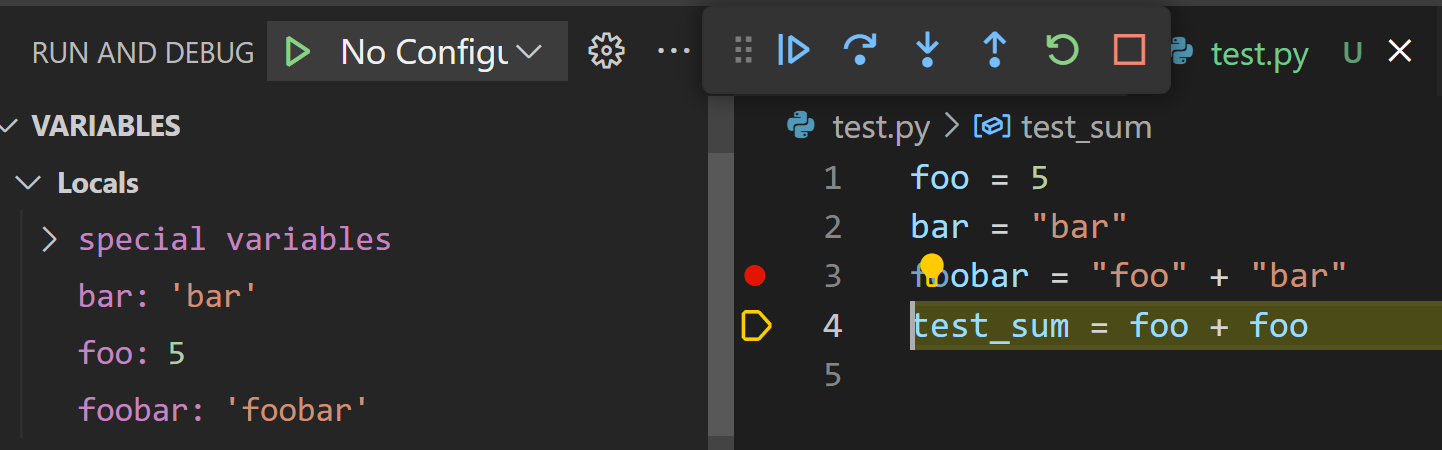
\includegraphics[scale=0.3]{imagenes/VScodeDebugger.png}
	\caption{Visual Studio Code Debugger.}
	\label{VScodeDebugger}
\end{figure}

Hay otros juegos cuya interfaz sirvió de inspiración para la realización del juego final, como 7 Billion Humans\cite{7billionhumans}, donde el código se ve a la derecha de la pantalla. La porción que contiene los elementos y eventos del juego está al lado izquierdo. Lo que ocurre en la interfaz de la derecha afecta al mundo virtual, tal como en la aplicación IGASCE.

\begin{figure}[h]
	\centering
	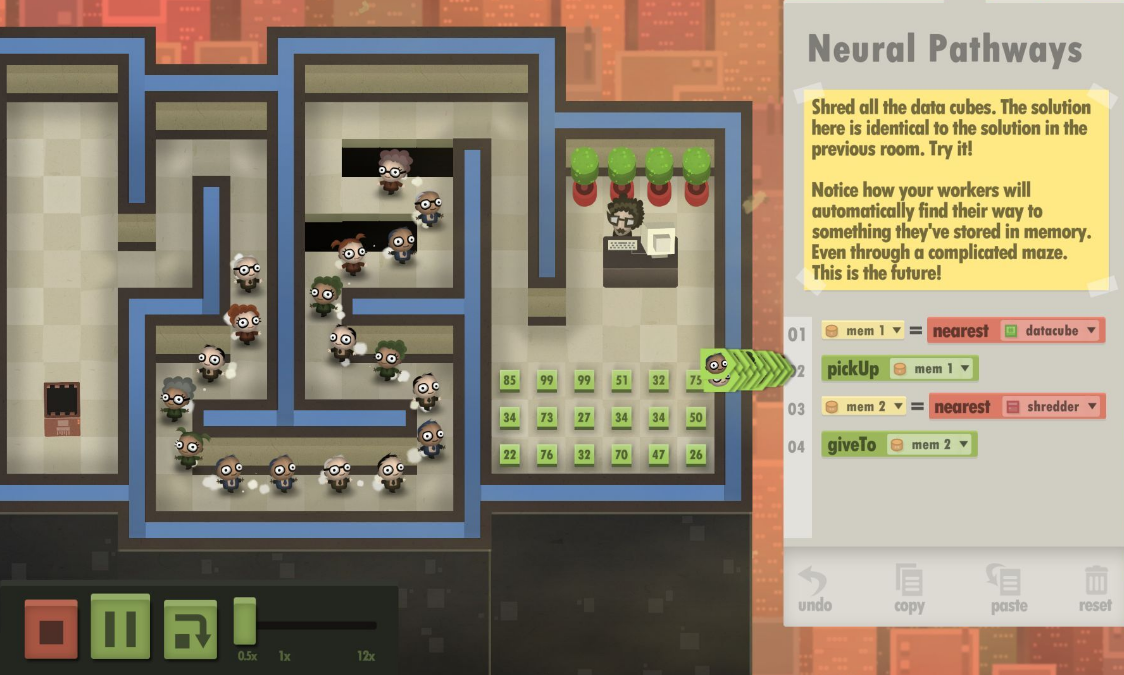
\includegraphics[scale=0.3]{imagenes/7BillionHumans.png}
	\caption{Videojuego 7 Billion Humans}
	\label{7BillionHumans}
\end{figure}


Otro videojuego con una interfaz similar es CodeCombat \cite{CodeCombat}. Aquí el código también está a la derecha, mientras que abajo se ven diálogos y elementos seleccionables. En el caso de IGASCE, los diálogos también se muestran abajo, así como las variables actuales y la seleccionada.
Además, el menú del juego se accede en la esquina superior izquierda (Ver figura \ref{CodeCombat}).

\begin{figure}[h]
	\centering
	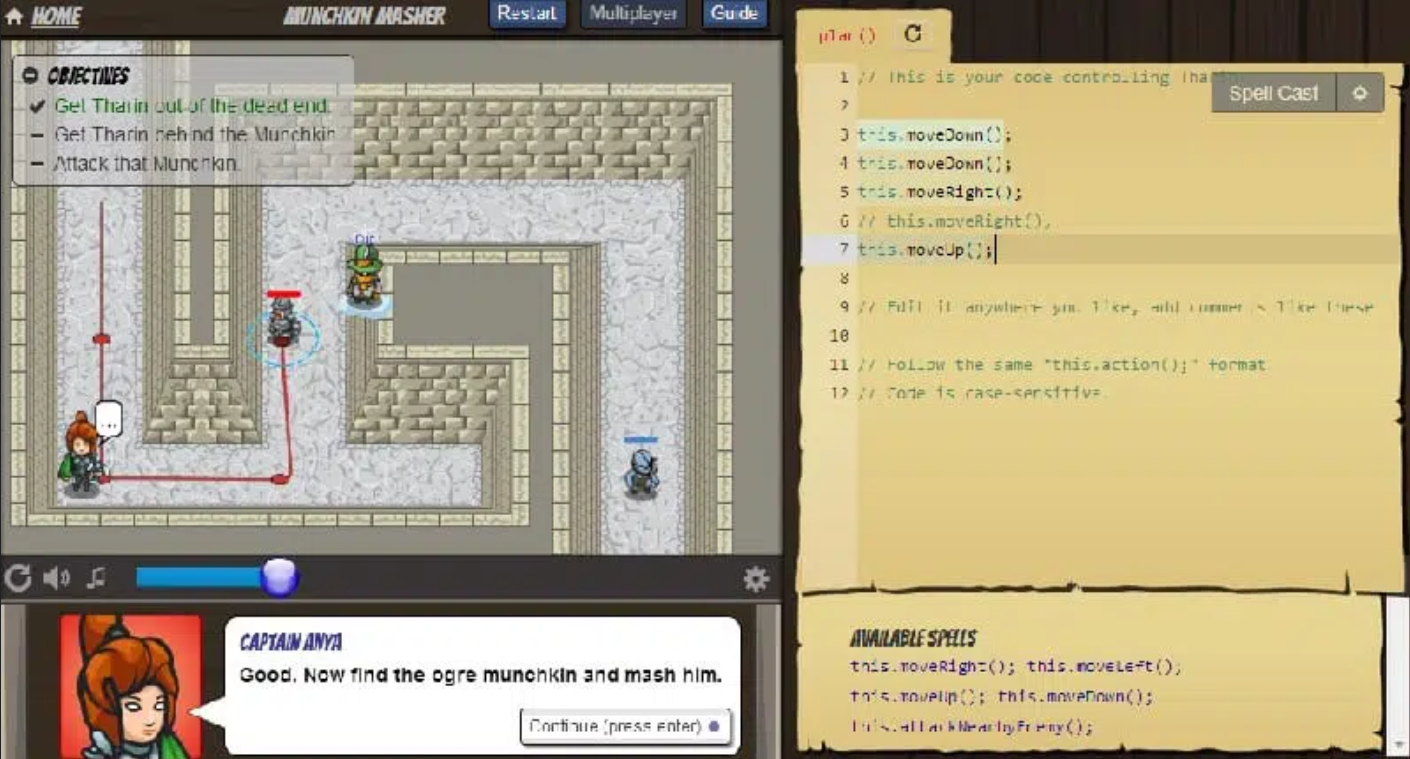
\includegraphics[scale=0.3]{imagenes/CodeCombat.png}
	\caption{Videojuego CodeCombat}
	\label{CodeCombat}
\end{figure}


\subsection{Diseño de efectos de sonido y música}

Los juegos retro comúnmente emplean bucles de música de 8 a 16 bits. Ejemplos notables incluyen Golden Sun \cite{Wiki_Golden_Sun}, ProtoCorgi \cite{ProtoCorgi}, Pokemon Emerald \cite{PokemonEmerald}, Space Invaders \cite{SpaceInvaders}, y Final Fantasy IV \cite{FinalFantasyIV}.

En juegos como Pokemon \cite{PokemonEmerald} y Golden Sun \cite{Wiki_Golden_Sun}, cada vez que se hace click en algún botón y se gatilla un evento, se emite un sonido de confirmación, como cuando el jugador selecciona un ataque. El objetivo es confirmarle al usuario que se está ejecutando correctamente una acción. IGASCE sigue una estrategia similar, utilizando sonidos agudos de confirmación al hacer clic en planetas, caminos o al presionar teclas correctamente (espacio o R). Estos sonidos nítidos cumplen la función de validar la ejecución exitosa de una acción sin distraer al jugador.

En contraste, los sonidos de error en IGASCE emplean tonos graves con desvanecimiento, generando una sensación de vibración (ver figura \ref{EspectroOndasSonidoError}). Estos sonidos más intensos se activan cuando el jugador comete errores, como hacer clic en un planeta incorrecto o un camino equivocado, presionar una tecla antes de completar una instrucción, o responder incorrectamente a preguntas del tipo Sí/No. La intención es que el jugador reconozca inmediatamente los errores y tome medidas correctivas.

\begin{figure}[h]
	\centering
	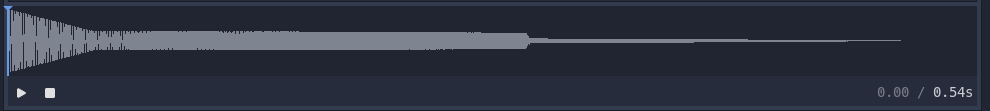
\includegraphics[width=0.9\textwidth]{imagenes/EspectroOndasConfirmacion.png}
	\caption{Espectro de Ondas del sonido de Confirmación de IGASCE}
	\label{EspectroOndasSonidoConfirmacion}
\end{figure}


\begin{figure}[h]
	\centering
	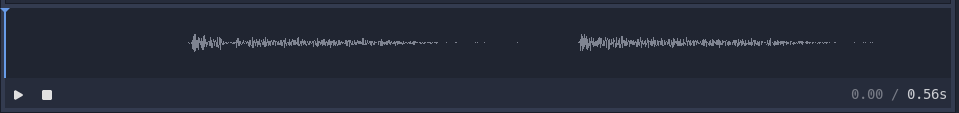
\includegraphics[width=0.9\textwidth]{imagenes/EspectroOndasError.png}
	\caption{Espectro de Ondas del sonido de Error de IGASCE}
	\label{EspectroOndasSonidoError}
\end{figure}


\subsection{Diseño de mecánicas de juego}

% Agregar diagrama de jugabilidad
La condición de victoria en cada nivel implica completar todas las instrucciones proporcionadas por el algoritmo. En los niveles de BFS y DFS, esto implica visitar todos los nodos del grafo. El puntero de instrucciones señala la tarea actual, y el jugador debe ejecutar correctamente lo indicado en la instrucción, ya sea haciendo clic, respondiendo una pregunta, o agregando un nodo a una estructura de datos. Algunas instrucciones, especialmente aquellas que contienen la palabra clave \textit{for}, no requieren acción por parte del jugador. Una vez que se han ejecutado correctamente los pasos requeridos, la instrucción cambiará de color y el cursor se transformará en un ticket.

Para avanzar en las instrucciones, el jugador debe presionar la tecla espacio. Si se presiona la tecla espacio sin completar la instrucción, se activará un sonido de error y el color de la instrucción parpadeará entre rojo y amarillo durante un segundo. Presionar la tecla espacio después de completar la instrucción generará un sonido de confirmación y avanzará a la siguiente instrucción. Si se presiona la tecla espacio cuando no hay más instrucciones, se emitirá un sonido de victoria, permitiendo al jugador pasar al siguiente nivel o visualizar los créditos según corresponda. Este proceso se resume en el diagrama \ref{FlujoMecanicaDeNivel}.

\begin{figure}[h]
	\centering
	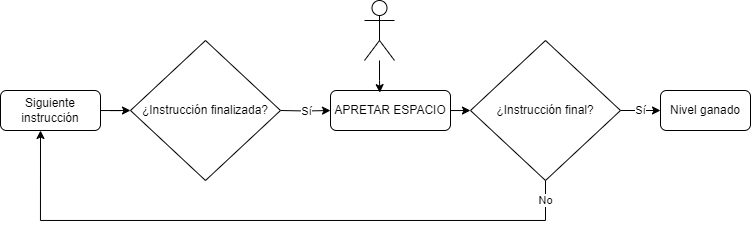
\includegraphics[width=0.9\textwidth]{imagenes/FlujoDeMecanicasDeNivel.drawio.png}
	\caption{Flujo de mecánicas de Nivel. El jugador debe seguir las instrucciones paso a paso.}
	\label{FlujoMecanicaDeNivel}
\end{figure}



\section{Arquitectura de software}

Antes de abordar la arquitectura específica del programa, es crucial comprender cómo se estructuran los programas en Godot. Esta comprensión sirve como base para justificar las decisiones de diseño adoptadas durante el desarrollo de la aplicación.

\subsection{Arquitectura de una aplicación en Godot}

Una aplicación en Godot se construye en base a escenas. Una escena es un conjunto de objetos instanciados al mismo tiempo. Un programa creado en este motor se compone de escenas, que típicamente serán los niveles en un juego. Las escenas tienen un grafo de escena compuesto por uno o más nodos.

Los nodos en Godot son las unidades fundamentales de construcción del programa, representando diversos elementos como botones, texturas, reproductores de sonido o áreas de colisión. Para crear personajes con lógica compleja, como habilidades, movimiento y colisiones, se combinan múltiples nodos.

La estructura del grafo de escena es beneficiosa en el desarrollo de videojuegos, ya que mover el nodo principal de un personaje implica automáticamente el movimiento de elementos asociados, como colisiones, sonidos y texturas. Esto simplifica la manipulación de elementos relacionados.

Otra ventaja clave de Godot es la capacidad de utilizar variables exportadas. Estas variables, cuyos valores se definen desde el editor, permiten instanciar objetos de la misma clase con características distintas \cite{GodotExportVariables}.

En comparación, trabajar a un nivel más bajo con bibliotecas como PyGame, que emplea OpenGL, requiere abordar individualmente cada aspecto de la representación de un objeto. Por ejemplo, mover un personaje implica gestionar texturas y colisiones por separado en el código, aumentando costos y complejidad de desarrollo \cite{GodotCollisionsAndRendering}.

\subsection{Arquitectura de software de la aplicación IGASCE}

La aplicación se desarrolla en diferentes fases, las cuales abarcan tres tipos de escenas: menús, tutoriales y niveles jugables. Cada fase hace uso de módulos distintos, y cada nivel, menú o tutorial representa una escena.

Los menús se construyen principalmente mediante nodos de control, comúnmente utilizados para interfaces gráficas. En este contexto, los menús consisten principalmente en botones que ejecutan códigos específicos según su descripción, dispuestos en formato vertical o en forma de grilla (Ver figura \ref{GodotMenuInterface}).

\begin{figure}[h]
	\centering
	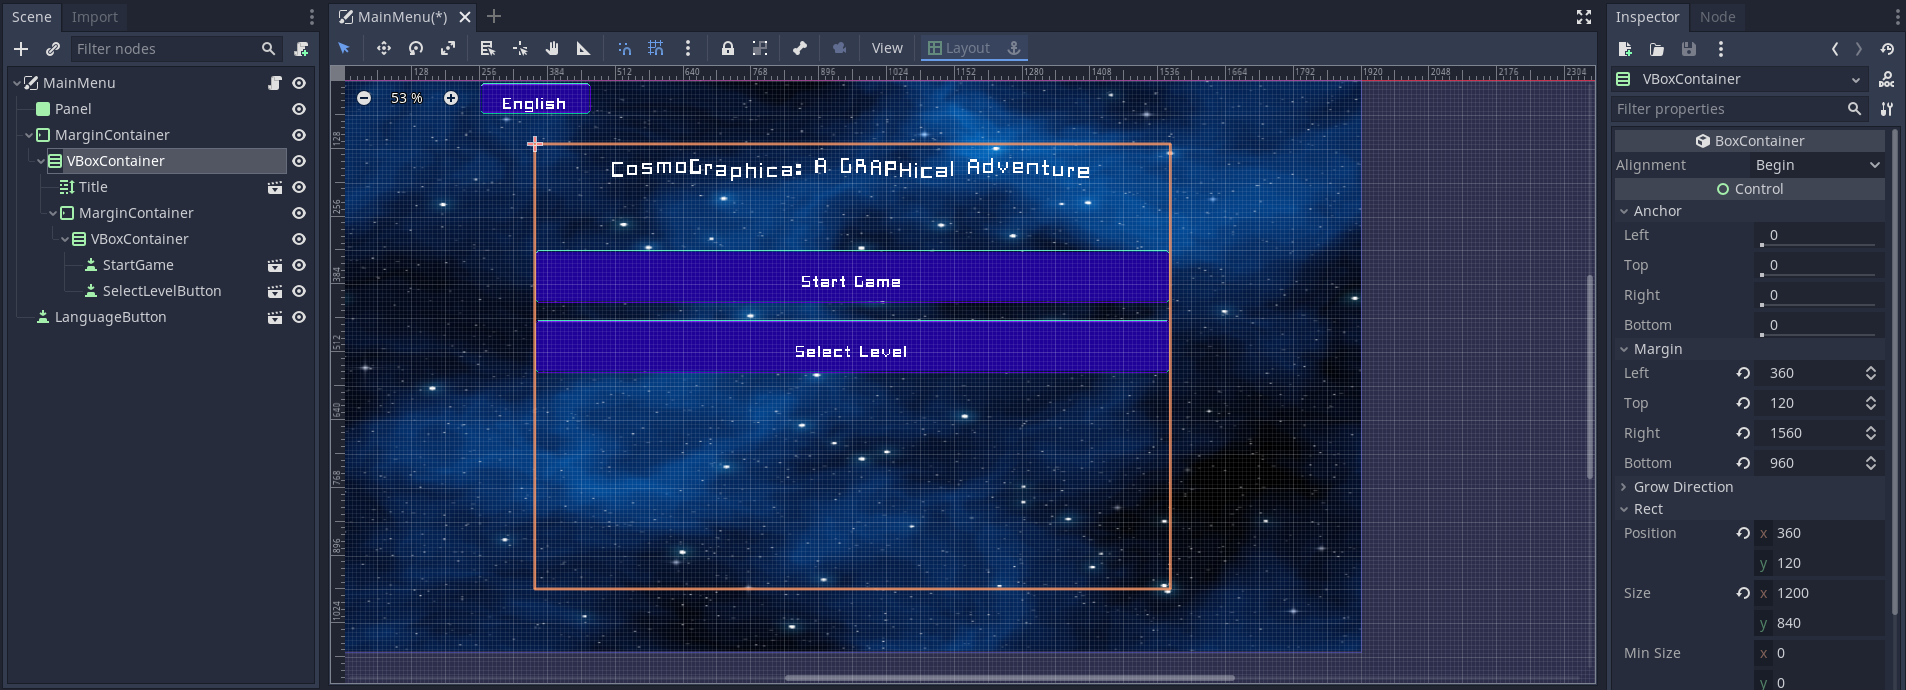
\includegraphics[width=0.9\textwidth]{imagenes/GodotInterfaceMainMenu.png}
	\caption{Interfaz de Godot describiendo la escena del menú principal de IGASCE. El juego públicamente se dio a conocer como CosmoGraphica, pero el proyecto completo se llama IGASCE.}
	\label{GodotMenuInterface}
\end{figure}


Los tutoriales presentan una lógica más compleja y se asemejan a los niveles. A diferencia de las escenas finales, los tutoriales incorporan una ventana de diálogo que busca vincular la historia del videojuego con los elementos interactivos. Además, en los tutoriales, el grafo ya está predefinido, lo que significa que los nodos y arcos ya están establecidos de antemano.

\begin{figure}[h]
	\centering
	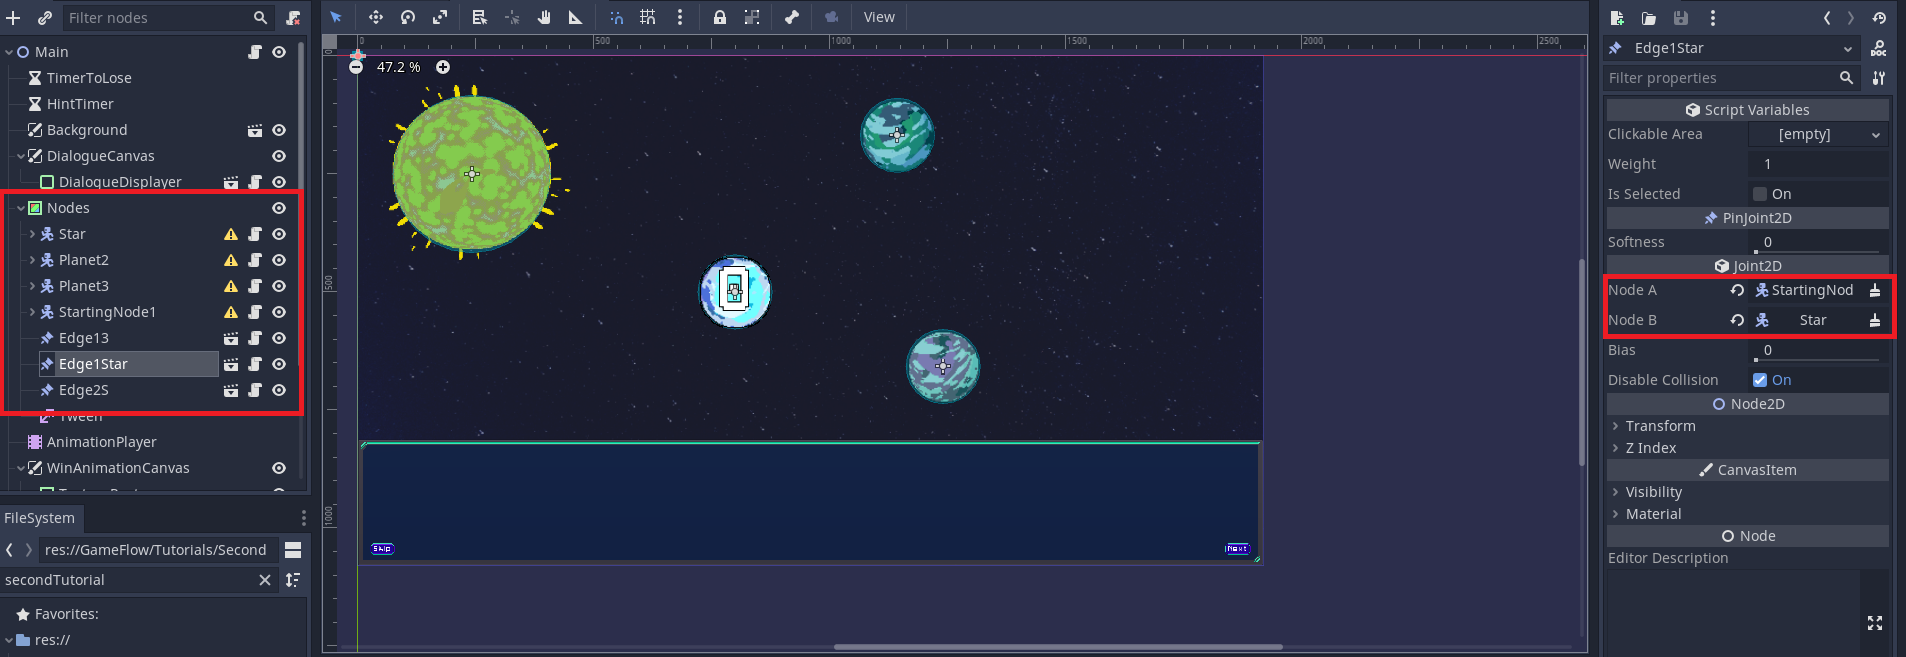
\includegraphics[width=0.9\textwidth]{imagenes/SecondTutorialGraph.png}
	\caption{Interfaz de Godot describiendo el segundo tutorial. En rojo se observa el grafo de escena con los nodos y los arcos ya predefinidos a la izquierda. En la derecha se muestra cómo se unen los arcos, indicando los dos extremos del arco a través de variables exportadas de Godot.}
	\label{SecondTutorialGraph}
\end{figure}


En cuanto a los niveles jugables, hay varios elementos destacables, como el código, las variables, la variable seleccionada y la ventana de juego.

El código que se muestra a la derecha de la pantalla durante el juego está controlado por un nodo de la clase CodeContainer. Este objeto se encarga de recibir la entrada del jugador para avanzar en el código. Si las acciones ejecutadas son correctas, el usuario pasa a la siguiente instrucción, desbloqueando nuevas tareas. La clase CodeContainer posee un arreglo de objetos del tipo CodeLine llamado code\_lines. La clase CodeLine contiene toda la lógica de una única línea de código. Entre sus funciones se encuentran dar énfasis a la línea de código actual, proporcionar feedback al usuario cuando la instrucción de la línea se completa correctamente y verificar constantemente si la instrucción de línea se ha completado correctamente (ver figura \ref{CodeLinesArchitecture}).

\begin{figure}[h]
	\centering
	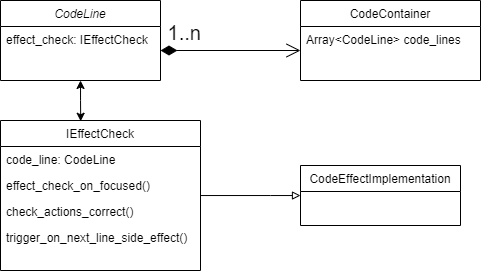
\includegraphics[width=0.9\textwidth]{imagenes/CodeLinesArchitecture.png}
	\caption{Arquitectura de software encargada de la mecánica de ejecución de código dentro del juego.}
	\label{CodeLinesArchitecture}
\end{figure}

Cada CodeLine posee un script que se puede indicar desde el editor de Godot a través de una variable exportada. Este script debe heredar de la clase EffectCheck, la cual actúa como interfaz. Cada script que implemente la interfaz EffectCheck debe definir métodos para: 1) cuando el puntero de instrucción llega a la línea del script; 2) verificar que la instrucción actual se ha realizado correctamente; y 3) si es necesario, manejar efectos colaterales de la instrucción. Este último se utiliza en los ciclos for, donde se mueve el índice utilizado para avanzar por los ciclos y recorrer arreglos, así como para la creación de variables.

En el panel inferior, se encuentran dos clases esenciales: DebugBlock y ADTShower. DebugBlock se encarga de mostrar las variables instanciadas, su nombre y su valor actual. Contiene la lógica para agregar, modificar o eliminar alguna variable. Cada vez que se pasa por un ciclo for o se declara una variable, este ajusta sus variables internas. Hay una variable seleccionada que puede ser manipulada por el usuario de diversas maneras. Al presionar la flecha hacia arriba, se selecciona la variable que está encima de la actual y viceversa para la flecha hacia abajo. En la figura \ref{BFSFullGame}, se observa que la variable ``q'' está seleccionada.

\begin{figure}[h]
	\centering
	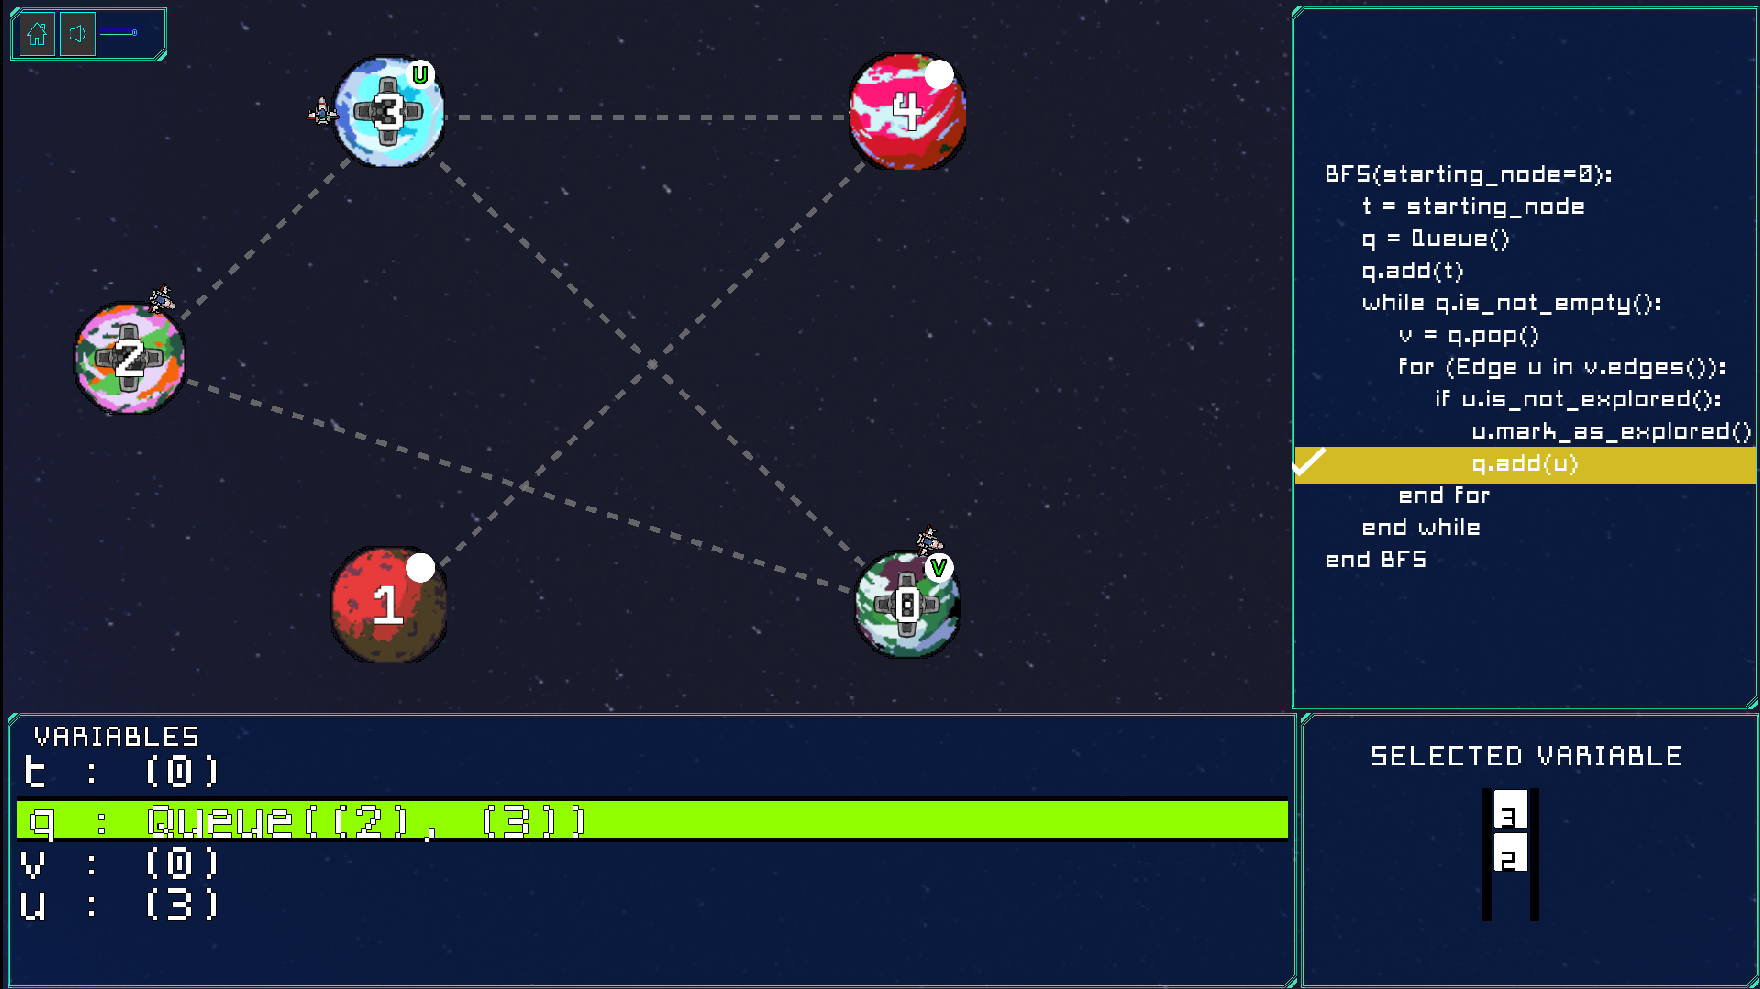
\includegraphics[width=0.9\textwidth]{imagenes/BFSFullGame.png}
	\caption{Nivel jugable BFS. Se observa el código a la derecha, el grafo en el centro, el DebugBlock en la parte inferior izquierda y el ADTShower en la esquina inferior derecha. La varible q está seleccionada.}
	\label{BFSFullGame}
\end{figure}

La clase ADTShower se encarga de mostrar en la esquina inferior derecha la variable que ha sido seleccionada por el usuario. Busca añadir una representación visual al objeto seleccionado para permitir arrastrar nodos a la cola o la pila según el algoritmo que se esté enseñando, BFS o DFS, respectivamente.

Inicialmente, cada cambio en el código debido al efecto de alguna CodeLine o línea de código del juego requería modificar las clases DebugBlock, ADTShower y StoredData (explicada más adelante), además de afectar la misma línea de código. Además, estos efectos deben reflejarse en las líneas de código siguientes para lograr cohesión. Por ejemplo, si la quinta línea crea la variable ``u'' y la sexta la modifica, esto se refleja correctamente en todas las estructuras mencionadas.

Para resolver el problema del alto costo de implementación, se optó por crear una clase llamada ADTMediator, siguiendo el patrón Mediator \cite{Freeman2015TheMP}. Esta clase se inspiró en la arquitectura de React, donde el código generado por React funciona como una única fuente de verdad o "Single Source of Truth" \cite{ReactSingleSourceOfTruth}. Con este tipo de arquitectura, se envía un mensaje a ADTMediator solicitando modificar, crear o eliminar una variable. Esta clase ajusta sus variables internas, luego informa a las clases DebugBlock y ADTShower sobre qué mostrar. Una desventaja de esta arquitectura es que realiza copias innecesarias en cada paso, perdiendo eficiencia. Sin embargo, dado que se trabaja con pocas variables, este costo no es notable a nivel de usuario.


\begin{figure}[h!]
	\centering
	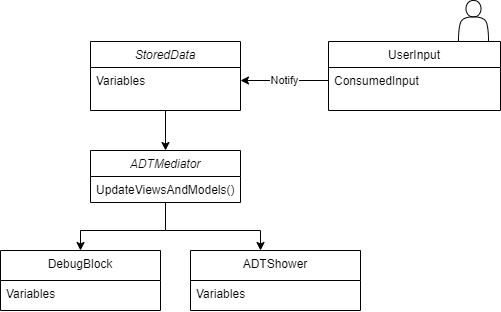
\includegraphics[width=0.9\textwidth]{imagenes/ArquitecturaMediatorAfter.png}
	\caption{Diagrama de un nivel utilizando el ADTMediator, reduciendo el acoplamiento entre clases.}
	\label{ArquitecturaMediatorAfter}
\end{figure}

Una clase que sirve de puente para comunicarse con el ADTMediator es StoredData. Este es un singleton que contiene datos como los avances del usuario en los distintos niveles y el estado del juego. Cuando una línea de código quiere modificar variables dentro del juego, ejecuta un método de este singleton, el cual reenvía esta información al ADTMediator. Esto se hace así porque es fácil obtener el puntero a StoredData, ya que usa el patrón singleton.

Otros singletons son: AudioPlayer, encargado de emitir sonidos específicos en cualquier momento del juego y NotificationManager, que genera ventanas emergentes para el usuario, como menúes, avisos o pestañas donde se debe responder sí o no.